\begin{figure*}[t]
    % \vspace{-5pt}
    \centering
    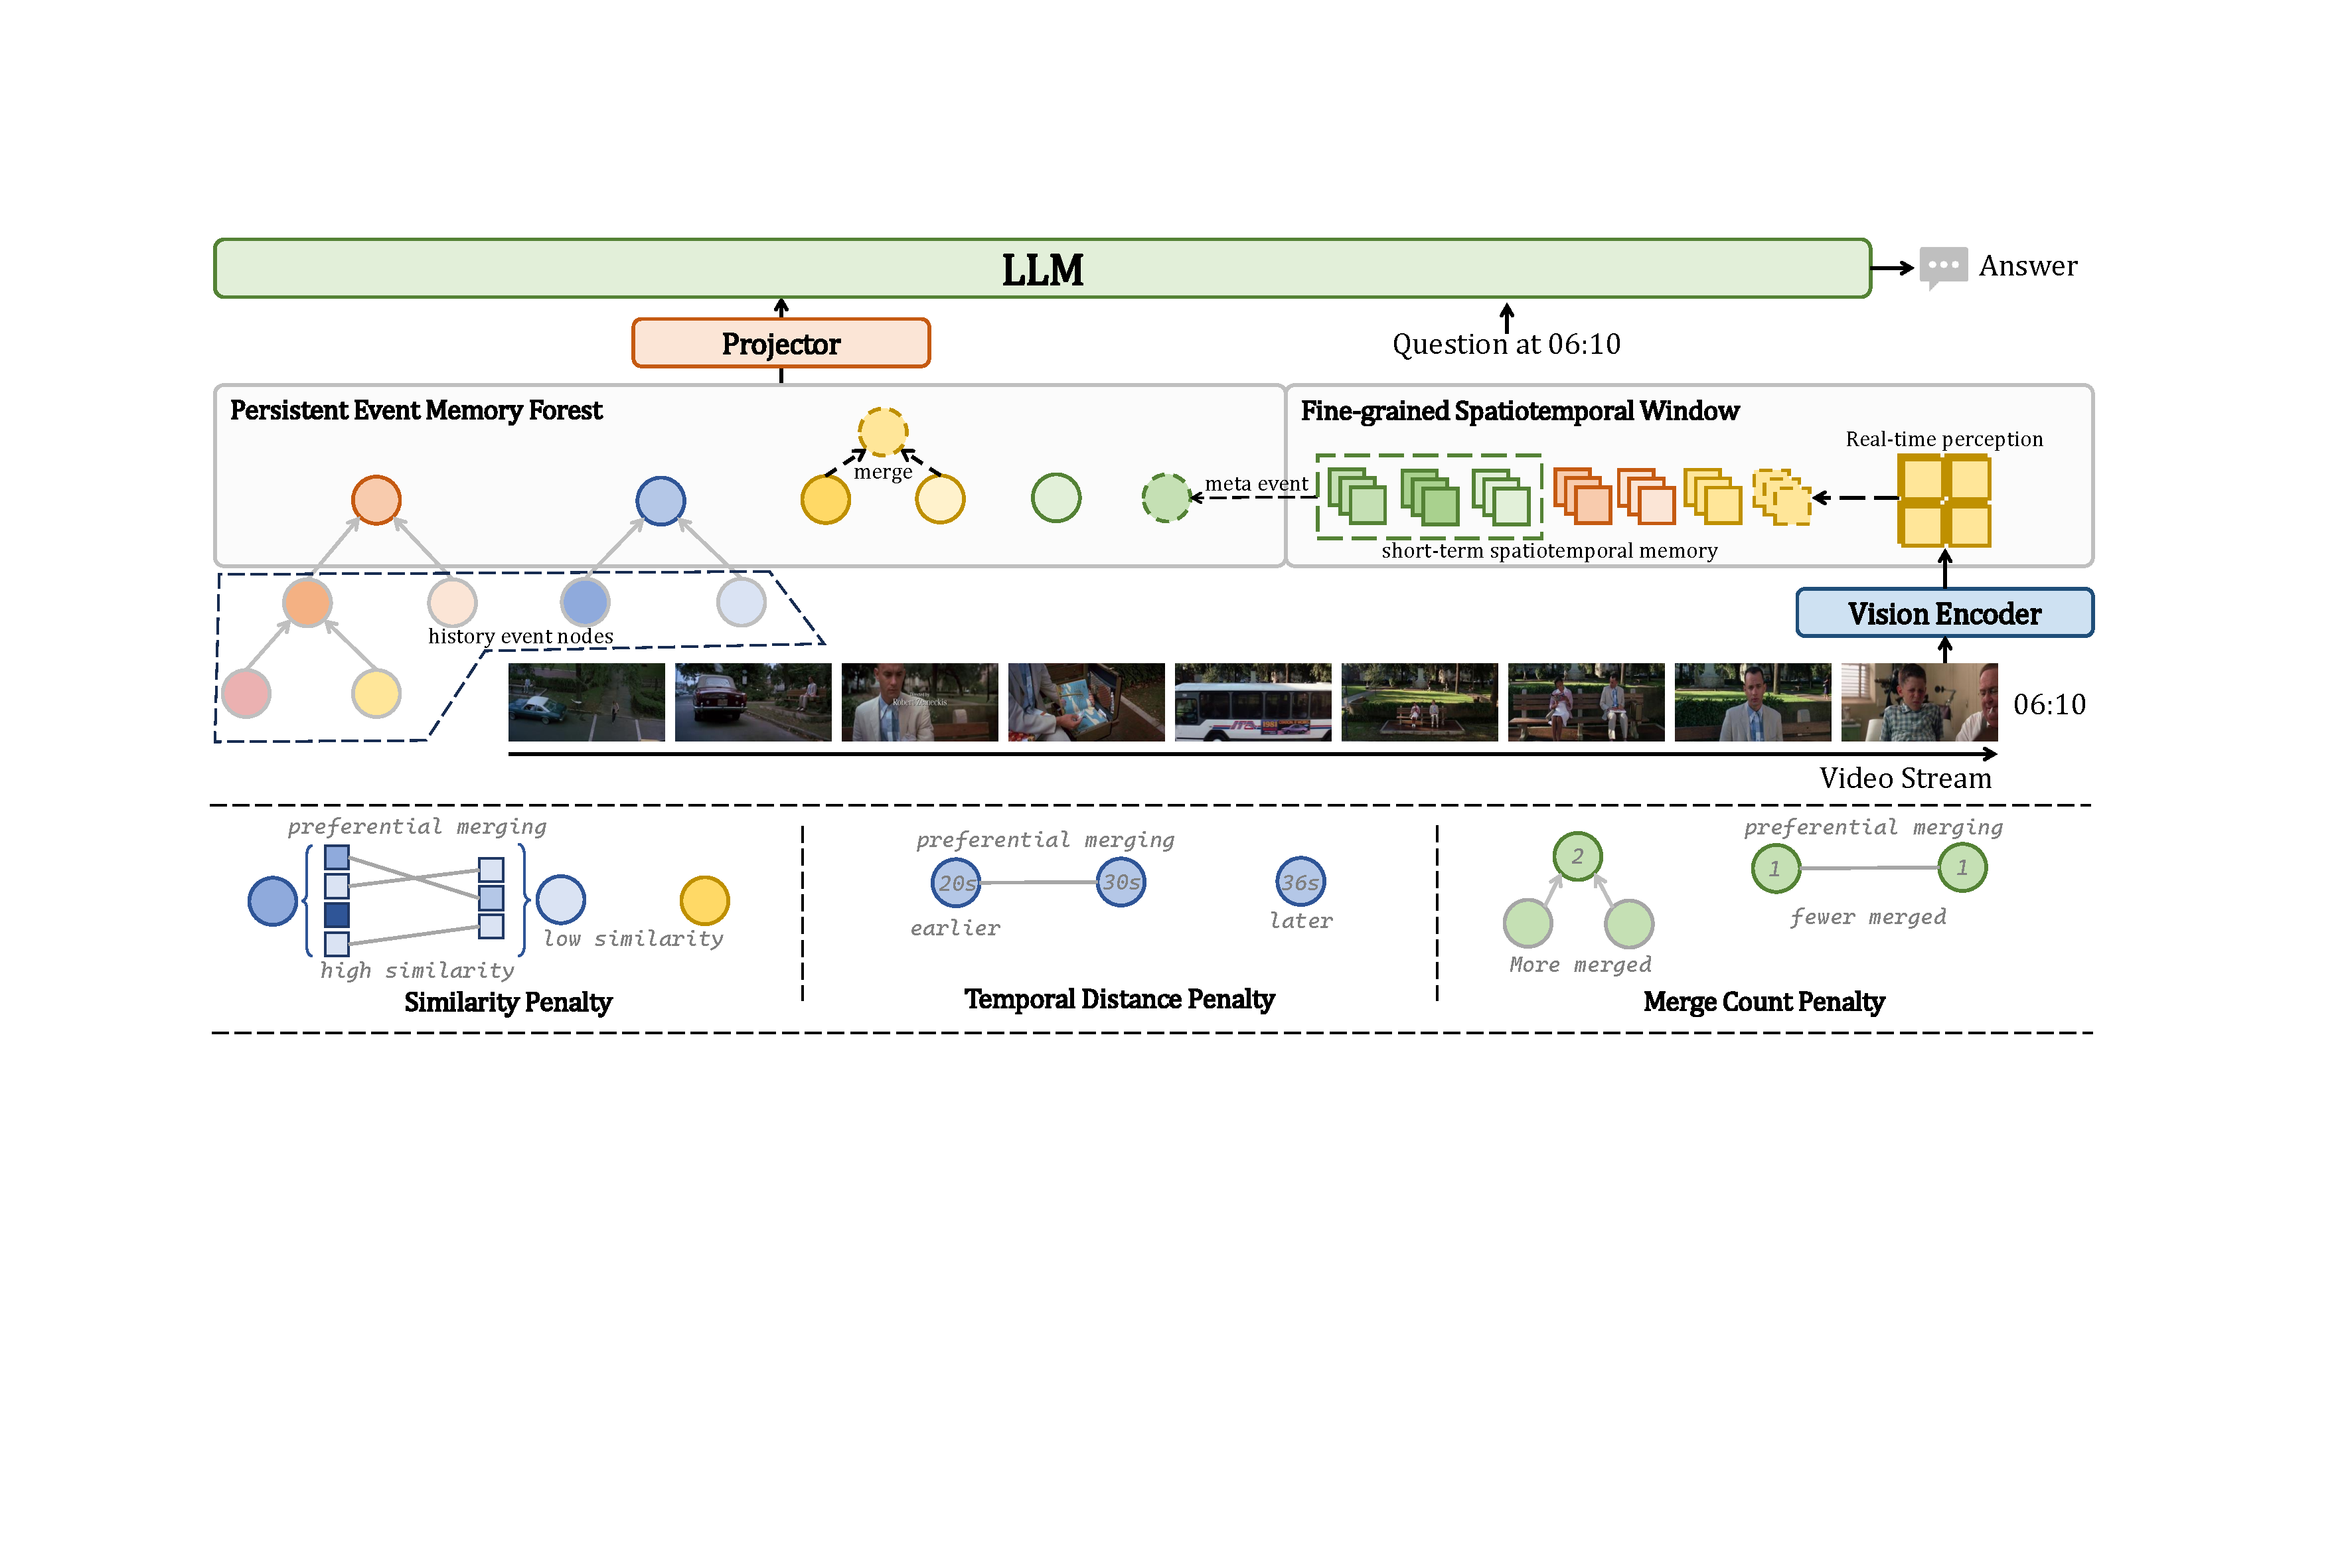
\includegraphics[width=\textwidth]{figs/architecture_img.pdf} 
    \caption{Visión general de nuestro StreamForest propuesto. La Fine-grained Spatiotemporal Window captura características espaciotemporales a nivel de instancia, mientras que la Persistent Event Memory Forest organiza adaptativamente representaciones a nivel de evento en un conjunto de estructuras arbóreas. Las flechas discontinuas y los feature tokens ilustran operaciones potenciales realizadas durante cada iteración de actualización de memoria.}
    \label{fig:architecture}
    % \vspace{-5pt}
\end{figure*}



% 图二：我们所提出的方法的架构示意图。流式记忆机制包含细粒度时空窗口和可持久化记忆森林。其中细粒度时空窗口用于建模实例级短期时空特征。而可持久化事件记忆森林自适应地将事件级特征簇组织成多个树形结构，以支持长程事件追溯。




% 我们提出的架构概览。记忆机制由两个互补的组件组成：时空细粒度窗口 (FSTW) 和持久事件记忆森林 (PEMF)。STFW 用于建模实例级短期时空特征，以应对流式视频理解应用场景的精准实时感知需求。PEMF自适应地将事件级特征组织成多个树形结构，以支持长程事件追溯。这两个模块共同使模型能够保持低延迟、高分辨率的感知，同时保留来自遥远过去的关键上下文信息。图中虚线标注的箭头与特征代表记忆在每次迭代更新时可能会执行的操作。


% \begin{figure}[h] % [h] 代表尽量放在当前位置
%     \centering
%     
\includegraphics[width=0.8\linewidth]{figures/framework.pdf} % 调整图片宽度
%     \caption{motivation}
%     \label{fig:single_column} % 为图片设置引用标签
% \end{figure}
